	\documentclass[10pt,oneside]{CBFT_book}
	
	% Algunos paquetes
	\usepackage{amsmath}
	\usepackage{amssymb}
	\usepackage{graphicx}
	\usepackage{libertine}
	\usepackage{lipsum}
	\usepackage[numbers]{natbib}
	\setcitestyle{square}


	\usepackage{polyglossia}
	\setdefaultlanguage{spanish}

	\usepackage{CBFT.estilo} % Cargo la hoja de estilo
	

	% Tipografías
	% \setromanfont[Mapping=tex-text]{Linux Libertine O}
	% \setsansfont[Mapping=tex-text]{DejaVu Sans}
	% \setmonofont[Mapping=tex-text]{DejaVu Sans Mono}

	%===================================================================
	%	DOCUMENTO PROPIAMENTE DICHO
	%===================================================================

% \title{CBFT Mecánica clásica}
% \author{Mecánica lagrangiana}
% \date{\today}

\begin{document}
% \maketitle
% \tableofcontents
\chapter{Conceptos de mecánica newtoniana}

Tal vez sea una simplificación, pero no una muy terrible, decir que el curso de mecánica clásica
busca reemplazar la mecánica basada en las ecuaciones de Newton,
\[
	\vb{F} = m \vb{a} 
\]
por un \emph{formalismo} más poderoso y que se podrá aplicar luego a otros campos.
Este formalismo constituye el corazón de la mecánica clásica.

El contenido de este capítulo forma un núcleo básico de los resultados de le mecánica newtoniana que necesitaremos 
tener a mano para lo subsiguiente (leyes de conservación del momento lineal, momento angular y energía) así como 
ciertos rudimentos mínimos de la matemática usual en la resolución de los problemas.

% =================================================================================================
\section{Leyes de conservación}
% =================================================================================================

Repasaremos a continuación las leyes de conservación fundamentales de la mecánica para sistemas de partículas.

\subsection{Momento lineal}

La segunda ley de Newton se podía escribir en función del momento lineal de una partícula de masa $ m $ como
\[
	\dtot{\vb{p}}{t} = \vb{F}
\]
siendo $ \vb{p} = m\vb{v} $ el momento de la partícula y $ F $ la fuerza total que actuaba sobre la misma.
Si el resultado de las fuerzas sobre la partícula era nulo entonces se tiene que $ \vb{p} = cte. $ (el momento lineal 
es una constante de movimiento).

En el caso de un sistema de $N$ partículas como el mostrado en la Figura \ref{fig_mc_leyes_cons} el momento total del 
sistema es la suma de los momentos individuales, es decir
\[
	\vb{P} = \Sum{i=1}{N} \vb{p}_i = \Sum{i=1}{N} m_i \vb{v}_i = \Sum{i=1}{N} m_i \dtot{\vb{x}_i}{t}
\]
luego la segunda ley para el sistema serán las $ N $ ecuaciones
\[
	\dtot{\vb{P}}{t} = \Sum{i=1}{N} m_i \dtot[2]{\vb{x}_i}{t} = \Sum{i=1}{N} \vb{F}_i
\]
donde $ \vb{F}_i$ es la fuerza total sobre la partícula $i$-ésima que puede descomponerse según
\be
	\vb{F}_i = \vb{F}_i^\text{ext} + \Sum{ j \neq i }{N} \vb{F}_{ij}
	\label{descomp_fuerzas}
\ee
siendo $ \vb{F}_i^\text{ext} $ las fuerzas debidas a agentes externos y $\vb{F}_{ij}$ la fuerza sobre la partícula $i$ 
debido a la partícula $j$.

\begin{figure}[hbt]
	\begin{center}
	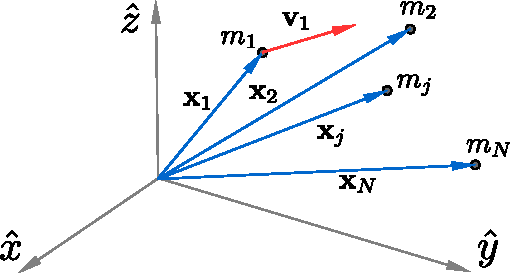
\includegraphics[width=0.6\textwidth]{images/fig_mc_leyes_cons.pdf}
	\end{center}
	\caption{Sistema de partículas de masas $m_i$ con sus correspondientes vectores de
	posición $\vb{x}_i$. La partícula $m_1$ tiene además indicado su vector velocidad $\vb{v}_1$.}
	\label{fig_mc_leyes_cons}
\end{figure} 

Entonces 
\[
	\dtot{\vb{P}}{t} = \Sum{i=1}{N} m_i \dtot[2]{\vb{x}_i}{t} = \Sum{i=1}{N} \vb{F}_i^\text{ext} + 
	\Sum{i=1}{N} \Sum{ j \neq i }{N} \vb{F}_{ij}
\]
pero el último término del RHS es nulo puesto que por cada sumando $ \vb{F}_{ij} $ también aparece el sumando 
$ \vb{F}_{ji} $ y por acción y reacción estas fuerzas tienen la misma dirección y sentido opuesto, i.e.
\[
	\vb{F}_{ij} = - \vb{F}_{ji}.
\]

De esta forma la ley de conservación para el sistema es 
\[
	\dtot{\vb{P}}{t} = \Sum{i=1}{N} \vb{F}_i^\text{ext} = \vb{F}^\text{ext}_\text{total}
\]
y el momento $ \vb{P} $ del sistema se conserva si la resultante de todas las fuerzas externas es nula. 

Definiendo el vector de posición del centro de masa como 
\[
	\vb{x}_\text{cm} = \frac{\sum_i m_i \vb{x}_i }{\sum_i m_i} = \frac{\sum_i m_i \vb{x}_i }{M}
\]
donde $ M $ es la masa del sistema, se tiene el resultado clásico de que
\[
	\dtot{}{t}( M \vb{x}_\text{cm} ) = \Sum{i=1}{N} m_i \vb{v}_i = M \vb{v}_\text{cm} = \vb{P},
\]
el sistema como un todo tiene un momento total que puede asociársele al de una única partícula {\it centro de masa} de 
masa $M$ y que se mueve con velocidad $ \vb{v}_\text{cm} $.

Si $\vb{P}$ se conserva, entonces $ \vb{v}_\text{cm} $ es una constante, el sistema posee un punto (el centro de masas) 
que se mueve con velocidad constante sin importar qué tan complejo sea el movimiento del conjunto total.

% ~~~~~~~~~~~~~~~~~~~~~~~~~~~~~~~~~~~~~~~~~~~~~~~~~~~~~~~~~~~~~~~~~~~~~~~~~~~~~~~~~~~~~~~~~~~~~~~~~~~~~~~~~~~~~~~~~~~~~
\subsection{Momento angular}

El momento angular de una partícula con momento lineal \vb{p} es 
\[
	\vb{l} = \vb{x} \times \vb{p} = m \: \vb{x} \times \vb{v}
\]
como puede verse en la Figura \ref{fig_mc_mom_ang_particula}. 
La variación temporal del momento angular,
\[
	\dtot{\vb{l}}{t} = \dtot{\vb{x}}{t} \times \vb{p} + \vb{x} \times \dtot{\vb{p}}{t} 
\]
se reduce al segundo término, puesto que $ d\vb{x}/dt = \vb{v} $ es paralela a $ \vb{p} $, y
se tiene finalmente el resultado conocido
\be
	\dtot{\vb{l}}{t} = \vb{x} \times \dtot{\vb{p}}{t} = \vb{x} \times \vb{f} = \vb{\tau}
	\label{conserv_mom_ang}
\ee
de que la variación del momento angular es el torque $\vb{\tau}$ causado por la fuerza $ \vb{f} $ 
que actúa sobre la partícula.

\begin{figure}[hbt]
	\begin{center}
	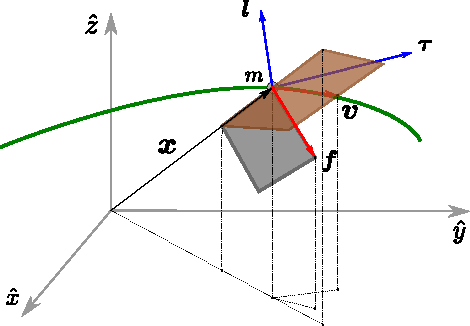
\includegraphics[width=0.6\textwidth]{images/fig_mc_mom_ang_particula.pdf}	
	\end{center}
	\caption{Una partícula de masa $m$ se desplaza en una trayectoria. En un punto \vb{x} de la misma se
	indican su velocidad \vb{v}, su momento angular \vb{l} y la fuerza \vb{f} a la que está sometida y el
	torque resultante \vb{\tau} por esa fuerza.
	El momento angular es perpendicular al plano (en marrón) definido por los vectores \vb{x} y \vb{v} mientras que 
	el torque los es al plano (en gris) definido por \vb{x} y \vb{f}.}
	\label{fig_mc_mom_ang_particula}
\end{figure} 

Dado que la definición de $ \vb{l} $ y de $ \vb{\tau} $ implica el vector de posición $ \vb{x} $ se sigue que ambas 
magnitudes dependen de la elección del origen del sistema de coordenadas. 
Es decir que una determinación de $ \vb{l} $ y $ \vb{\tau} $ tiene sentido únicamente con respecto a un cierto origen 
de coordenadas.

De la ecuación \eqref{conserv_mom_ang} se deduce que si la fuerza es siempre paralela al vector de posición de una 
partícula ($\vb{f} \parallel \vb{x}$) entonces el momento angular \vb{l} se conserva puesto que el torque es 
$\vb{\tau}=0$ en ese caso. Es lo que se llama una fuerza central.
\notamargen{Habría que destacar lo de fuerza central con un dibujo. Es importante.}

\subsubsection{Momento angular para un sistema de partículas}

Si ahora tenemos un sistema de $N$ partículas el momento angular correspondiente (con respecto a un dado origen de
coordenadas) será
\[
	\vb{L} = \Sum{i=1}{N} \: \vb{x}_i \times \vb{p}_i
\]

De manera equivalente, la variación temporal es 
\[
	\dtot{\vb{L}}{t} = \Sum{i=1}{N} \vb{x}_i \times \vb{f}_i
\]
y si utilizamos la descomposición \eqref{descomp_fuerzas} para la fuerza $\vb{f}_i$ resulta
\[
	\dtot{\vb{L}}{t} = \Sum{i=1}{N} \vb{x}_i \times \vb{F}_i^\text{ext}  +
	\Sum{i=1}{N} \Sum{j\neq i}{N}  \vb{x}_i \times \vb{F}_{ij}
\]

Es claro\footnote{Nota \ref{nota_suma_ineqj}} que el segundo término puede expresarse de manera equivalente como 
\[
	\Sum{i=1}{N} \Sum{j\neq i}{N}  \vb{x}_i \times \vb{F}_{ij} =
	\frac{1}{2} 
	\Sum{i=1}{N} \Sum{j \neq i}{N}  \left[ \vb{x}_i \times \vb{F}_{ij} + \vb{x}_j \times \vb{F}_{ji} \right]
\]
y aceptando que las fuerzas internas son pares acción-reacción se tiene 
\[
	\Sum{i=1}{N} \Sum{j\neq i}{N}  \vb{x}_i \times \vb{F}_{ij} =
	\frac{1}{2} 
	\Sum{i=1}{N} \Sum{j \neq i}{N}  \left[ \vb{x}_i - \vb{x}_j \right] \times \vb{F}_{ij},
\]
de manera que la derivada del momento angular total es 
\be
	\dtot{\vb{L}}{t} = \Sum{i=1}{N} \vb{x}_i \times \vb{F}_i^\text{ext}  +
	\frac{1}{2} \Sum{i=1}{N} \Sum{j \neq i}{N}  \left[ \vb{x}_i - \vb{x}_j \right] \times \vb{F}_{ij} 
	\label{dL_sistema}
\ee

La conservación de \vb{L},
\[
	\dtot{\vb{L}}{t} = 0	
\]
requiere entonces que las fuerzas externas sean centrales (lo cual anula el primer término en \eqref{dL_sistema}) y que 
se verifique 
\[
	\vb{F}_{ij}  \parallel ( \vb{x}_i - \vb{x}_j ),
\]
es decir que la fuerza sobre $i$ ejercida por la partícula $j$ tenga la dirección del vector que une las dos 
partículas, para anular el segundo término de \eqref{dL_sistema}.

\begin{figure}[htb]
	\begin{center}
	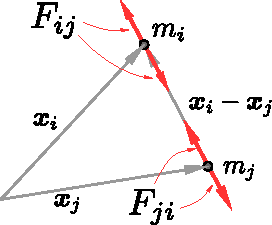
\includegraphics[width=0.4\textwidth]{images/fig_mc_parstrong.pdf}	
	\end{center}
	\caption{Principio de acción y reacción fuerte para dos partículas de masas $m_i$ y $m_j$.}
	\label{fig_mc_parstrong}
\end{figure} 

Esto establece lo que se llama un ``principio de acción y reacción {\it fuerte}''; las fuerzas son iguales y opuestas 
(de esto se trata el principio de acción y reacción), pero además colineales.
Dadas dos partículas del sistema cualesquiera con posiciones $ \vb{x}_i, \vb{x}_j $ y de masas $ m_i, m_j $, como se 
muestra en la Figura \ref{fig_mc_parstrong}, la fuerza $\vb{F}_{ij}$ sobre $i$ debido a $j$ debe estar contenida en la 
dirección del vector $ \vb{x}_i - \vb{x}_j $ lo cual le otorga las dos posibilidades indicadas por las flechas rojas 
gruesas. Para la fuerza $\vb{F}_{ji}$ el razonamiento es, por supuesto, idéntico.

\notamargen{Acá hay más para extraer: poner un gráfico con lo que no puede pasar. Poner un código de colores para
las flechas, puesto que si son iguales y opuestas las fuerzas están hermanadas las externas por un lado y las internas
por el otro.}

La existencia de un principio de acción y reacción fuerte sobreviene por la naturaleza puntual de los cuerpos. De no 
ser puntuales se tendrá principio de acción y reacción a secas.

Existe otras descomposición interesante para el momento angular \vb{L} de un sistema de $N$ partículas en términos de 
sus distancias al centro de masas.

Para cada partícula $i$-ésima con posición $ \vb{x}_i $ y velocidad $ \vb{v}_i $ definimos una coordenada $ \vb{x}_i' $ 
y una velocidad $\vb{v}_i' $ en términos de la posición \vb{R} y velocidad \vb{V} del centro de masa, ver Figura 
\ref{fig_mc_angularmom}, de acuerdo a
\[
	\vb{x}_i = \vb{R} + \vb{x}_i' \qquad \vb{v}_i = \vb{V} + \vb{v}_i'
\]

\begin{figure}[hbt]
	\begin{center}
	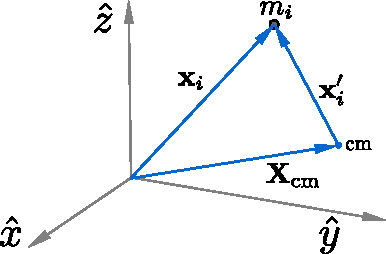
\includegraphics[width=0.6\textwidth]{images/fig_mc_angularmom.pdf}	
	\end{center}
	\caption{}
	\label{fig_mc_angularmom}
\end{figure} 

En términos de estas nuevas variables primadas el momento angular es
\[
	\vb{L}_O = \Sum{i=1}{N} \vb{x}_i \times \vb{p}_i = 
	\Sum{i=1}{N} (\vb{R} + \vb{x}_i') \times m_i (\vb{V} + \vb{v}_i')
\]
\[
	\vb{L}_O = \Sum{i=1}{N} ( \vb{R} \times m_i \vb{V}  + \vb{R} \times m_i \vb{v}_i'
	+ \vb{x}_i' \times m_i \vb{V} 	+ \vb{x}_i' \times m_i \vb{v}_i' )
\]

Como la posición del centro de masa es
\be
	\vb{R} = \frac{1}{M} \Sum{i=1}{N} m_i \vb{x}_i  
	\label{R_cm}
\ee
se tendrá 
\[
	M \vb{R} = \Sum{i=1}{N} m_i \vb{x}_i = \Sum{i=1}{N} m_i ( \vb{R} + \vb{x}_i' ) =
	\vb{R} \Sum{i=1}{N} m_i + \Sum{i=1}{N} m_i \vb{x}_i'
\]
pero el primer término del RHS es $M\vb{R}$ de manera que 
\be
	\Sum{i=1}{N} m_i \vb{x}_i' = 0 .
	\label{Condicion_cm}
\ee
La velocidad del centro de masa es la derivada temporal de \eqref{R_cm}, i.e.
\be
	\vb{V} = \frac{1}{M} \Sum{i=1}{N} m_i \dtot{\vb{x}_i}{t} = 
	\frac{1}{M} \Sum{i=1}{N} m_i \vb{v}_i
	\label{V_cm}
\ee

Con estos resultados volvemos a la expresión del momento que resulta 
\[
	\vb{L}_O = \vb{R} \times M \vb{V}  + \vb{R} \times \left( \Sum{i=1}{N} m_i \vb{v}_i' \right) +
	\left( \Sum{i=1}{N} m_i \vb{x}_i' \right) \times \vb{V} + \Sum{i=1}{N} \vb{x}_i' \times m_i \vb{v}_i',
\]
pero debido a \eqref{Condicion_cm} y a su derivada temporal (que resulta nula) el segundo y tercer sumando de la 
expresión anterior son nulos y entonces 
\[
	\vb{L}_O = \left( \vb{R} \times M \vb{V} \right) + \Sum{i=1}{N} ( \vb{x}_i' \times m_i \vb{v}_i' )
\]
% \[
% 	\vb{L}^T_O = \vb{L}^{cm} + \vb{L}^{sist}_{cm}
% \]
siendo el primer término del RHS el momento angular orbital y el segundo el momento angular de spin.

% Con respecto a la conservacion del momento angular, se tendrá
% \[
% 	\dtot{\vb{L}_O}{t} = \sum \vb{\tau}_O
% \]
% que se puede ver como suma del torque de fuerzas externas y de fuerzas internas. En el primer caso,
% los torques externos sumarán cero si las fuerzas externas son nulas o centrales.
% En el segundo caso los torques internos son nulos si vale el principio de acción y reacción fuerte;
% es decir si
% \[
% 	\vb{r}_i - \vb{r}_j \parallel F_{ij}.
% \]

% ~~~~~~~~~~~~~~~~~~~~~~~~~~~~~~~~~~~~~~~~~~~~~~~~~~~~~~~~~~~~~~~~~~~~~~~~~~~~~~~~~~~~~~~~~~~~~~~~~~~~~~~~~~~~~~~~~~~~~
\subsection{Trabajo y energía}

Consideremos una partícula de masa $ m $ que se mueve sobre una cierta trayectoria suave $\vb{x}(t)$, ver {Figura} 
\ref{fig_mc_workenergy}, debido a la acción de una fuerza \vb{F}.
Su velocidad \vb{v} es en todo momento tangente a la trayectoria y define de esta forma un versor $ \hat{t} $
colineal con la misma. Esto define un plano, mostrado en la parte derecha de la figura, para el cual todo vector
perteneciente al mismo es normal a la trayectoria. Elegimos un versor $ \hat{n} $ que está en la dirección de
la proyección de \vb{F} sobre dicho plano.

\begin{figure}[!h]
	\begin{center}
	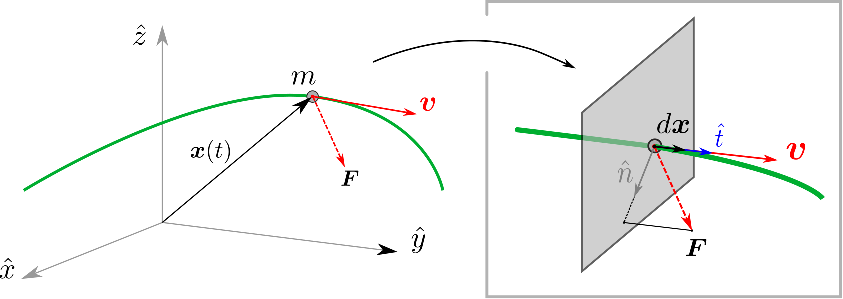
\includegraphics[width=0.9\textwidth]{images/fig_mc_workandenergy.pdf}	
	\end{center}
	\caption{Partícula de masa $m$ que se mueve sobre una trayectoria $\vb{x}(t)$ bajo la acción de una fuerza 
\vb{F} (izquierda). En el detalle de la derecha se muestra la descomposición del movimiento en direcciones
tangencial $\hat{t}$ y normal $\hat{n}$.}
	\label{fig_mc_workenergy}
\end{figure} 

Descomponiendo la fuerza y la velocidad en estas dos direcciones, se tiene 
\[
	\vb{F} = F^t \: \hat{t}  + F^n \: \hat{n} \qquad \qquad \vb{v} = v \: \hat{t}
\]
de manera que la segunda ley de Newton, 
\[
	m \: \dtot{\vb{v}}{t} = \vb{F},
\]
para la componente $\hat{t}$ resulta
\[
	m \dtot{v}{t} = F^t
\]
\notamargen{Notemos que el versor desplazamiento $d\vb{s}$ {\it camina} por la trayectoria.}
Involucrando al diferencial de arco $ ds = | d\vb{x} | $ a lo largo de la trayectoria, la ecuación anterior se
puede escribir como
\be
	m \: dv \:\dtot{s}{t} = m \: v \: dv = F^t \: ds = \vb{F} \cdot d\vb{x},
	\label{ec_trabajo}
\ee
donde la última igualdad es posible en virtud de que $ F^n \perp d\vb{x} $ por construcción.

Podemos integrar ambos miembros de \eqref{ec_trabajo} entre $\vb{x}(t_0) \equiv \vb{x}_0$ y su 
correspondiente velocidad $v(t_0) \equiv v_0$ hasta $\vb{x}_1, \vb{v}_1$, 
\[
	m \int_{v_0}^{v_1} \: v \: dv = \int_{\vb{x}_0}^{\vb{x}_1}  \vb{F} \cdot d\vb{x}
\]
obteniendo
\[
	\left. \frac{1}{2} m v^2 \right|_{v_0}^{v_1} = W_{\vb{x}_0 \to \vb{x}_1} 
\]
que es el llamado \emph{teorema de las fuerzas vivas} para una partícula de masa $m$ y nos dice que la
variación de energía cinética en la trayectoria es igual al trabajo de todas las fuerzas que actúan
sobre la misma, i.e.
\be
	T_1 - T_0 = \Delta T_{\vb{x}_0 \to \vb{x}_1}  = W_{\vb{x}_0 \to \vb{x}_1} .
	\label{conser_energia}
\ee

En el caso particular en que la fuerza sea normal a la trayectoria en todo el intervalo $[t_0,t_1]$ se 
tendrá $\Delta T = 0 $, es decir que se conserva la energía cinética a lo largo de toda la trayectoria.
Sólo las componentes tangenciales de la fuerza producen trabajo y esto es solamente debido a que este proviene
de un producto escalar (una proyección); las componentes normales no hacen trabajo.

\notamargen{ Falta meter lo de \[ 	 m \frac{v^2}{\rho} = F_n \] }

Si la fuerza proviene de un potencial\footnote{El menos delante del gradiente es una convención, como se verá a
continuación}, se tiene 
\be
	\vb{F} = - \nabla V
	\label{fuerza_prov_potencial}
\ee
y podemos expresar en coordenadas cartesianas esta equivalencia \eqref{fuerza_prov_potencial}
\[
	\vb{F} = -\left( \dpar{V}{x_1}, \dpar{V}{x_2}, \dpar{V}{x_3} \right)
\]
y evaluar la integral del trabajo para obtener
\[
	W = \int_{\vb{x}_0}^{\vb{x}_1}  \vb{F} \cdot d\vb{x} =
	\int_{t_0}^{t_1}  \vb{F}(\vb{x}[t]) \cdot \dotvb{ x } \: dt =
	- \int_{t_0}^{t_1}  \sum_{i=1}^3 \left[ \dpar{V}{x_i} \dtot{x_i}{t} \right] \: dt = V_0 - V_1
\]
donde la última igualdad se obtiene por integración de un gradiente. Esto 
significa que la integral es independiente de la trayectoria $\vb{x}_0 \to \vb{x}_1$.

Entonces, volviendo a \eqref{conser_energia}
\[
 	\rlap{ $\overbrace{\phantom{T_1 - T_0 = W_{0 \to 1}}}^{\text{Vale siempre}} $}  T_1 - T_0 =
	\underbrace{ W_{0 \to 1} = V_0 - V_1 }_{\text{Si $\vb{F}$ proviene de potencial} }
\]
y pasando de miembros se tiene 
\[
	(T_1 + V_1) = (T_0 + V_0 ) 
\]
que viene a significar que la cantidad $ E = T + V $ (la energía mecánica) se conserva si la fuerza $\vb{F}$ 
proviene de un potencial $V$. 
Por dicha razón, las fuerzas para las cuales se verifica \eqref{fuerza_prov_potencial} se llaman {\it fuerzas
conservativas}. En una dimensión, cualquier $ F(x) $ se puede hacer provenir de un potencial si verifica ser
integrable, es decir si podemos definir
\be
	V(x) = \int F(x) \: dx.
	\label{potencial_1d}
\ee
Para tres dimensiones no cualquier $ F(\vb{x}) $ es conservativa.

El signo negativo en \eqref{fuerza_prov_potencial} hace que la cantidad conservada sea $T+V$ en lugar de $T-V$.
Tiene más sentido físico que se conserve una suma de energías antes que una resta de las mismas.

\subsubsection{Trabajo y energía para un sistema de partículas}

Para un sistema de $ N $ partículas la energía cinética simplemente es la suma de las energías cinéticas de cada 
partícula,
\[
	T = \sum_{i=1}^N \: \frac{1}{2} \: m_i v_i^2.
\]

La definición del trabajo, en cambio, es un poco más complicada. Entre dos instantes de tiempo $ t $ y $ t + \Delta t $ 
el sistema está caracterizado por las $ N $ posiciones $ \{\vb{x}_i\} $ de todos sus integrantes y cada partícula 
experimenta un desplazamiento $ \Delta \vb{x}_i $ asociado con la fuerza que actúa sobre ella.

En principio la fuerza sobre cada partícula puede dividirse en interna (debida a las otras partículas del sistema) y 
externas (debida a agentes exteriores al sistema), lo cual permite escribir
\[
	\vb{F} = \vb{F}^{\text{int}} + \vb{F}^{\text{ext}}
\]
y consecuentemente
\[
	W = W^{\text{int}} + W^{\text{ext}}
\]

El $ W $ entre dos instantes de tiempo $t_0$ y $t_1$ corresponde ahora a la integral entre la configuración del sistema 
a $t_0$ dada por $ \{\vb{x}_i(t_0)\} $ hasta la configuración $ \{\vb{x}_i(t_1)\} $, las cuales etiquetaremos como 0 y 
1 respectivamente. 

Entonces el trabajo externo es
\[
	W^{\text{ext}} = \sum_{i=1}^N \int_0^1 \vb{F}^{\text{ext}}_i \cdot \: d\vb{x}_i
\]
siendo $ \vb{F}^{\text{ext}}_i $ la fuerza externa sobre la partícula $i$. Para que valga la conservatividad es 
necesario que 
\begin{itemize}
 \item La fuerza sobre $i$ dependa solamente de las coordenadas $\vb{x}_i$ de esa partícula. Es decir:
 \[
	\vb{F}_i = \vb{F}_i(\vb{x}_i)
 \]
 \item Se verifique para cada $\vb{F}_i$ 
 \[
	\Nabla \times \vb{F}_i = 0,
 \]
 donde el operador $\nabla$ se toma con respecto a las coordenadas de la partícula $i$ en cuestión.
\end{itemize}

\begin{figure}[!h]
	\begin{center}
	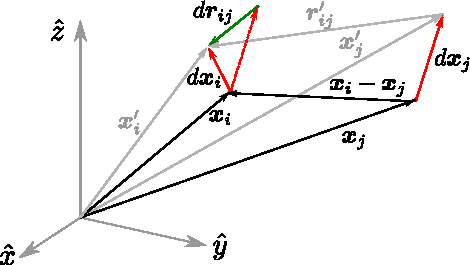
\includegraphics[width=0.75\textwidth]{images/fig_mc_work_system.pdf}	
	\end{center}
	\caption{Elementos implicados en la evaluación del trabajo interno $ W^{\text{int}} $ para un sistema
	de partículas.}
	\label{fig_mc_work_system}
\end{figure} 

Estas condiciones permiten escribir la fuerza como el gradiente de un potencial y entonces el trabajo externo es la 
suma de las diferencias entre las energías potenciales de las partículas entre las configuraciones 0 y 1, o bien
\[
	W^{\text{ext}} = - \sum_{i=1}^N \left. \Delta V_i(\vb{x}_i) \right|_0^1
\]

El trabajo interno corresponde a la suma sobre cada partícula $i$ de la fuerza ejercida por todas las otras partículas 
$j \neq i$ del sistema, es decir
\be
	W^{\text{int}} = \sum_{i=1}^N \sum_{j\neq i}^N \int_0^1 \vb{F}_{ij} \cdot d\vb{x}_i
	\label{internal_work}
\ee
donde $\vb{F}_{ij} $ es la fuerza sobre $i$ ejercida por $j$. La restricción en la sumatoria sobre $j$ descarta la suma 
de autofuerzas. Es claro que la expresión \eqref{internal_work} se puede escribir equivalentemente como
\[
	\frac{1}{2} \sum_{i=1}^N \sum_{j\neq i}^N \int_0^1 
	\left( \vb{F}_{ij} \cdot d\vb{x}_i + \vb{F}_{ji} \cdot d\vb{x}_j \right) 
\]
\notamargen{¿nota final con la justificación de que se puede escribir así?}
% justificación :
% Esta sumatoria tiene N(N-1) términos que resultan de los N por N posibilidades excluyendo los N tales que i=j
% Por cada término del tipo F_ij dx_i hay un correspondiente F_ji dx_j; por ejemplo está F_13 dx_1 (i=1 u j=3) y F_31 
% dx_3 que viene de i=3 y j=1. Luego podemos sumar todo dos veces considerando un sumando general F_ijdx_i + F_jidx_j 
% preo dividiendo por dos para compensar. 
%
y si ahora aceptamos que vale el principio de acción y reacción
\[
	\frac{1}{2} \sum_{i=1}^N \sum_{j\neq i}^N \int_0^1 
	\vb{F}_{ij} \cdot \left(d\vb{x}_i - d\vb{x}_j \right) .
\]
Definiendo luego un vector de separación relativa $ \vb{r}_{ij} = \vb{x}_i - \vb{x}_j $ se tiene que las integrales son 
de la forma 
\[
	\int \vb{F}_{ij} \cdot d\vb{r}_{ij}
\]
y sabemos, por analogía con lo anterior, que si $\vb{F}_{ij}$ depende del vector de separación $ \vb{r}_{ij} $ y es de 
rotor nulo entonces las fuerzas internas son conservativas.
En estos casos
\[
	\Delta E = \sum_{i=1}^N ( \Delta T_i - \Delta V_i ) + \frac{1}{2} \sum_{i=1}^N \sum_{j=1}^N \Delta V_{ij}
\]

% ~~~~~~~~~~~~~~~~~~~~~~~~~~~~~~~~~~~~~~~~~~~~~~~~~~~~~~~~~~~~~~~~~~~~~~~~~~~~~~~~~~~~~~~~~~~~~~~~~~~~~~~~~~~~~~~~~~~~~
\begin{ejemplo}{\bfseries Análisis energético de un potencial }
\label{ejemplo_analisis_potencial}
Dada una fuerza 1D 
\[
	F(x) = -k x + \frac{a}{x^3}
\]
se realiza un análisis del potencial resultante y de la energía.

A partir de esta fuerza, que es la del oscilador armónico 1D sumada a una perturbación controlada por el parámetro 
$a$, procedemos a calcular el potencial, a través de la relación \eqref{potencial_1d} de modo que (a menos de una 
constante aditiva que no interesa aquí) se obtiene
\[
	V(x) = \frac{1}{2} k x^2 + \frac{1}{2} \frac{a}{x^2}
\]

% Para analizar el movimiento bajo este potencial consideraremos tres relaciones diferentes entre los parámetros $k,a$ 
% para poder graficar $ V(x) $. Consideraremos tres casos numéricos $ k = 100 a, 20 a, 5 a $ (dado que $k$ y $a$ son 
% magnitudes dimensionalmente diferentes es evidente que estos números 100, 20 y 5 tienen unidades, aunque no interesan 
% para este análisis).

Para analizar el movimiento bajo este potencial dividimos ambos miembros sobre $ a $ y definiendo un $\tilde{V} = V/a$
y consideraremos tres casos representativos $ k/a = 5, 20, 100 $. Este potencial $ \tilde{V} $ es una especie de 
potencial por unidad de $ a $ 

\end{ejemplo}




% =================================================================================================
\section{Definiciones}
% =================================================================================================

El número de grados de libertad es el número de coordenadas independientes para resolver el problema.
Las fuerzas de vínculo $F^v$ se {\it acomodan} en todo momento para satisfacer las ligaduras.
Entonces las $\vb{F}^v$ son perpendiculares a los desplazamientos compatibles con los vínculos de
manera que 
\[
	W_{F^v} = 0
\]
\begin{figure}[hbt]
	\begin{center}
	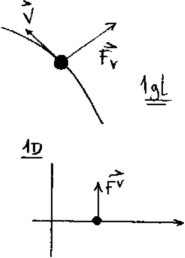
\includegraphics[width=0.3\textwidth]{images/fig_mc_vinculos1.pdf}	 
	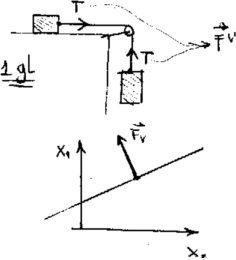
\includegraphics[width=0.3\textwidth]{images/fig_mc_vinculos2.pdf}
	\end{center}
	\caption{}
\end{figure} 

Los vínculos se clasifican en
\[
\textrm{holónomos} 
\begin{Bmatrix}
 f(r_i,t) = 0 \qquad \textrm{reónomos} \\
\; f(r_i) = 0 \qquad \textrm{esclerónomos} \;\\
\end{Bmatrix} 
\]
los cuales cumplen que  $W_{virtual}^{F^v}=0$, y
\[
\textrm{no holónomos} 
\begin{Bmatrix}
 f(r_i,t) \geq 0  \\
 f(r_i) \geq cte. \quad f(\dot{r}_i) = 0  \; \\
\end{Bmatrix}
\]
los cuales no cumplen, en general, que $\vb{F}^v$ perpendicular al desplazamiento posible.
\begin{figure}[hbt]
	\begin{center}
	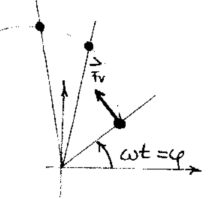
\includegraphics[width=0.3\textwidth]{images/fig_mc_vinculos3.pdf}	
	\end{center}
	\caption{}
\end{figure} 
donde un desplazamiento virtual es un desplazamiento a $t_0$ fijo compatible con los vínculos,
mientras que un desplazamiento real es un desplazamiento en $\delta t$ durante el cual varían
fuerzas y ligaduras.

A tiempo fijo el desplazamiento es en $\hat{r} \perp \vb{F}^v$.

\[
	f(x_i,t) = cte. \Longrightarrow \sum_i^N \dpar{f}{x_i} \delta x_i + \dpar{f}{t} \delta t = 0 
\]
o bien
\[
	\nabla f \cdot \vb{\delta r} = 0
\]

% =================================================================================================
\section{Sistemas de coordenadas}
% =================================================================================================

\subsection{Coordenadas polares}

La gran ventaja de las coordenadas cartesianas es que los versores $ \hat{i}, \hat{j}, \hat{k}$ no varían con el tiempo,
entonces
\[
	\vb{r}(t) = x \hat{i} + y \hat{j}
\]
lleva a que 
\[
	\vb{v} = \dtot{\vb{r}}{t} = \dot{x}\hat{i} + \dot{y}\hat{j}
\]
\[
	\vb{r} = r \:\hat{r}
\]
y la derivada temporal se hace con la regla de Leibniz
\[
	\dtot{\vb{r}}{t} = \dtot{r}{t} \:\hat{r} + r \:\dtot{\hat{r}}{t}
\]
y para evaluar la evolución temporal pasamos la expresión a cartesianas según
\[
	\hat{r} = \cos \varphi \:\hat{x} + \sin \varphi \:\hat{y}
\]
\[
	\hat{\varphi} = -\sin \varphi  \:\hat{x} + \cos  \varphi \:\hat{y}
\]

\[
	\dtot{\vb{r}}{t} = \dot{r} \hat{r } + r( - \sin \vp \dot{\vp} \:\hat{x} + \cos \vp \dot{\vp} \:\hat{y} )
\]
que se puede escribir como 
\[
	\dtot{\vb{r}}{t} = \dot{r} \: \hat{r } + r \dot{\vp} \: \hat{\vp} = \dot{\vb{r}}
\]
y extraemos de conclusión que 
\[
	\dtot{\hat{r}}{t} = \dot{\vp} \: \hat{\vp}
\]

Luego, para la aceleración hay que derivar la velocidad con respecto al tiempo
\[
	\ddot{\vb{r}} = \dtot{}{t} ( \dot{r} \hat{r} + r\dot{\vp} \hat{\vp} ) 
\]
\[
	\ddot{\vb{r}} = \dtot{\dot{r}}{t} \hat{r} + \dot{r}\dtot{\hat{r}}{t} + \dtot{r}{t} \dot{\vp} \hat{\vp}
	+ r \left( \dtot{\dot{vp}}{t}\phiver + \dot{\vp}\dtot{\phiver}{t} \right)
\]
\[
	\ddot{\vb{r}} = ( \ddot{r} - r\dot{\vp}^2 ) \rver + ( r\ddot{\vp} + 2 \dot{r} \dot{\vp} ) \phiver
\]
\subsection{Coordenadas esféricas}

\[
	\rver = \cos\vp \sin\theta\xver + \sin\vp\sin\theta\yver + \cos\theta\zver
\]
\[
	\phiver = -\sin\vp \xver + \cos\vp \yver
\]
\[
	\thetaver = \cos\theta \cos\vp \xver + \cos\theta\sin\vp\yver - \sin\theta\zver
\]

\[
	\vb{r} = r \rver
\]
\[
	\vb{v} = \dot{r} \rver + r\dot{\theta}\thetaver + r\dot{\vp}\sin\theta\phiver
\]
\begin{multline*} % No puedo usar \vb porque no se da cuenta que multline ES modo matemático
	\symbf{a} = ( \ddot{r} - r\dot{\theta}^2 - r\dot{\vp}^2 \sin^2 \theta )\rver +
	( r\ddot{\theta} + 2\dot{r}\dot{\theta} - r\dot{\vp}^2 \sin \theta \cos\theta )\thetaver + \\
	( r\ddot{\vp}\sin\theta + 2\dot{r}\dot{\vp}\sin\theta + 2r\dot{\theta}\dot{\vp}\cos\theta )\phiver 
\end{multline*}
	
\subsection{Rotación del sistema de coordenadas}

Un vector de acuerdo a dos sistemas de coordenadas en el plano,
\[
	\vb{A} = A_x\xver + A_y\yver \qquad \qquad \vb{A}' = A_x'\xver' + A_y'\yver'
\]
\[
	\left. \dtot{\vb{A}}{t} \right|_\text{inercial} = 
	\dot{A_x'}\xver' + \dot{A_y'}\yver' + A_x'\dot{\xver'} + A_y\dot{'\yver'}
\]
pero como la situación geométrica es la misma que la cuenta de polares, se tiene 
\[
	\dtot{\xver'}{t} = \dot{\theta} \yver' \qquad \qquad 
	\dtot{\yver'}{t} = -\dot{\theta} \xver'
\]

\[
	\left. \dtot{\vb{A}}{t} \right|_\text{fijo} = \left. \dtot{\vb{A}}{t} \right|_\text{móvil}
	+ A_x' \dot{\theta}\yver' - A_y'\dot{\theta}\xver'
\]
donde 
\[
	\left. \dtot{\vb{A}'}{t} \right|_\text{móvil} \equiv \sum_i \dtot{A_i'}{t} \: \hat{e_i}'
\]
\[
	\left. \dtot{\vb{A}}{t} \right|_\text{móvil} = \dot{A_x'}\xver' + \dot{A_y'}\yver'
\]
\[
	\vb{\omega} = \dot{\theta} \zver
\]
\[
	\vb{\omega}\times\vb{A}' = \dot{\theta} \times ({A_x'}\xver' + {A_y'}\yver') =
	A_x' \dot{\theta}\yver' - A_y'\dot{\theta}\xver'
\]
\[
	\left. \dtot{\vb{A}}{t} \right|_\text{fijo} = \left. \dtot{\vb{A}}{t} \right|_\text{móvil}
	+ \vb{\omega} \times \vb{A}'
\]
\[
	\left. \vb{v} \right|_\text{fijo} = \left. \vb{v} \right|_\text{móvil} + \vb{\omega} \times \vb{r}'
\]
\[
	\left. \vb{v} \right|_\text{móvil} = \dot{x'}\xver' + \dot{y}\yver' 
\]
\[
	\vb{a} = \left. \dtot{\vb{v}}{t} \right|_\text{fijo} = \left. \dtot{\vb{v}}{t} \right|_\text{móvil} +
	\vb{\omega} \times \dtot{\vb{r}}{t}
\]

\[
	\vb{a} = \dtot{}{t}\left[ \left. \dtot{\vb{r}}{t} \right|_\text{móvil} + \vb{\omega}\times\vb{r} \right] +
	\vb{\omega} \times \left[ \left. \vb{v} \right|_\text{móvil} +	\vb{\omega}\times\vb{r} \right]
\]

\[
	\dtot{}{t}\left.( \dot{x'}\xver' + \dot{y'}\yver' )\right|_\text{móvil} = 
	\ddot{x'}\xver' + \ddot{y'}\yver' \equiv \left. \vb{a} \right|_\text{móvil}
\]
\[
	\left.\vb{\omega}\times\vb{r}\right|_\text{móvil} = \omega y' \xver' - \omega x' \yver'
\]

\[
	\dtot{}{t}\left.\vb{\omega}\times\vb{r}\right|_\text{móvil} = 
	( \dot{\omega} y' + \omega \dot{y}' )\xver' + ( \dot{\omega} x' + \omega \dot{y'} )\yver'
\]
\[
	\left. \vb{a}\right|_\text{fijo} = \left. \vb{a}\right|_\text{móvil} +
	\dot{\omega}y'\xver'- \dot{\omega}x'\yver' + 2\vb{\omega}\times\vb{v'} + \vb{\omega}
	\times (\vb{\omega} \times \vb{r})
\]
donde el segundo término del RHS es $ \dot{\vb{\omega}} \times \vb{r}$, el tercero la aceleración de Coriolis y el 
cuarto la aceleración centrípeta.
Llamando $ \alpha = \dot{\omega} = \dtot{\omega}{t}$ resulta 
\[
	\vb{F} = m\vb{a} = m \left. \vb{a}\right|_\text{móvil} + m \alpha \times \vb{r} + 4m 
	\vb{\omega}\times\vb{v'}+m[  \vb{\omega} \times (\vb{\omega}\times\vb{r} )]
\]
que reacomodado de otra manera es 
\[
	\vb{F} - m \alpha \times \vb{r} - 4m \vb{\omega}\times\vb{v'} - m[\vb{\omega} \times(\vb{\omega}\times\vb{r})]
	= m \left. \vb{a}\right|_\text{fijo}
\]
y ahora en el LHS tenemos la fuerza $\vb{F}$ que es la única que produce par de acción y reacción, y los términos de 
fuerza lineal, de Coriolis y centrífuga.
Si $\omega = cte.$ entonces la fuerza lineal es nula.

% Como ejemplo citamos \cite{einstein}.
% O bien \cite{example}.
% Tal vez \citep{Aspnes:1973}

\begin{notasfinales}

\label{nota_suma_ineqj}
\item{ \bf Sumatoria de torques}
Una manera de convencerse de que esta escritura es posible es hacer un diagrama de los diferentes términos que
aparecen en esta doble sumatoria. Es fácil de ver que con el añadido del término $\vb{x}_j \times \vb{F}_{ji} $ se está 
haciendo un doble conteo que justifica el $1/2$ que aparece luego.

Una demostración más matemática puede lograrse escribiendo la sumatoria $ j\neq i $ sin esta restricción, lo cual se 
puede hacer así:
\[
	\Sum{i=1}{N} \Sum{j\neq i}{N}  \vb{x}_i \times \vb{F}_{ij} = 
	\Sum{i=1}{N} \Sum{j=1}{N}  \vb{x}_i \times \vb{F}_{ij} ( 1 - \delta_{ij} )
\]
siendo $ \delta_{ij} $ la delta de Kronecker. Es claro que podemos hacer un cambio de etiquetas en las sumatorias 
puesto que los índices sumados son {\it mudos}, i.e.
\[
	\Sum{i=1}{N} \Sum{j=1}{N}  \vb{x}_i \times \vb{F}_{ij} ( 1 - \delta_{ij} ) = 
	\Sum{j=1}{N} \Sum{i=1}{N}  \vb{x}_j \times \vb{F}_{ji} ( 1 - \delta_{ij} )
\]
y dado que el orden de las sumatorias es irrelevante llegamos a
\[
	\Sum{i=1}{N} \Sum{j\neq i}{N}  \vb{x}_i \times \vb{F}_{ij} = \frac{1}{2}
	\Sum{i=1}{N} \Sum{j=1}{N} \left[ \vb{x}_i \times \vb{F}_{ij} ( 1 - \delta_{ij} ) +
	\vb{x}_j \times \vb{F}_{ji} ( 1 - \delta_{ij} )
	\right] 
\]

Regresando ahora a las sumatoria restringida obtenemos 
\[
	\Sum{i=1}{N} \Sum{j\neq i}{N}  \vb{x}_i \times \vb{F}_{ij} = \frac{1}{2}
	\Sum{i=1}{N} \Sum{j \neq i }{N} \left[ \vb{x}_i \times \vb{F}_{ij} + \vb{x}_j \times \vb{F}_{ji} \right] 
\]
que es el resultado buscado.


\end{notasfinales}


% ============================================================================

% \bibliographystyle{CBFT-apa-good} % (uses file "apa-good.bst")
% \bibliography{CBFT.Referencias} % La base de datos bibliográfica


\end{document}
